% SOEN 6011 - Summer 2026 - Deliverable 2, Problems 5-7
% Student ID: 40324569 | Function F5: a*b^x
% Compile with: pdflatex d2_f5.tex   (run twice)
%
% screenshot1.png, screenshot2.png, screenshot3.png must sit in the same
% folder as this .tex file.
%
% MAIN TRACK: 13 slides (title + 12), target under 6 minutes.
% Everything after \appendix is APPENDIX material, shown on request.
%
% -----------------------------------------------------------------
% ACTION LIST BEFORE SUBMITTING - do not leave any of these unchecked
% -----------------------------------------------------------------
% [ ] A1. Confirm the repository URL below is exact and public.
% [ ] A2. Confirm f5_gui.py actually rejects "inf", "-inf" and "nan".
%         Python's float() ACCEPTS these strings, so a plain float()
%         call will let them through. FR-08 claims they are rejected.
%         If the code does not reject them, fix the code, not the slide.
% [ ] A3. Confirm f5_gui.py rejects an empty entry field (FR-07).
% [ ] A4. Re-run verify_f5.py and confirm the worst relative error is
%         still 4.6e-11 and that the table on the backup slide matches.
% [ ] A5. Check the footer slide count reads 13 on the main track.
% -----------------------------------------------------------------

\documentclass[11pt]{beamer}
\usetheme{Madrid}
\usecolortheme{seahorse}
\usepackage{booktabs}
\usepackage{graphicx}

\title[D2]{SOEN 6011: Deliverable 2 \\ Function F5: $f(x) = ab^{x}$ \\ Problems 5--7}
% Short forms in [] keep the Madrid footer inside the slide width.
% The long forms in {} are what appear on the title slide.
\author[C. Singh --- 40324569]{Chandanpreet Singh \\ Student ID: 40324569 \\ Function: F5 --- $ab^{x}$}
\date{Summer 2026}

\begin{document}

\begin{frame}
  \titlepage
\end{frame}

% ===============================================================
\begin{frame}{Response to D1 Feedback}
  \textbf{What the D1 evaluation said:} the demonstration ran too long and
  the answers were not short enough.
  \medskip

  \textbf{What I changed for D2:}
  \begin{itemize}
    \item Main track is 13 slides. Everything else is in the appendix.
    \item The demonstration is scripted and rehearsed: five cases, ninety seconds.
    \item Every number on a slide comes from a measurement I can show.
  \end{itemize}
  \medskip

  \textbf{What the marker asked for, and where it is answered:}
  \begin{itemize}
    \item Running out of iterations is no longer called an overflow
          (Exception Handling slide).
    \item Every requirement now traces to a uniquely identified persona
          element (Problem 7 slides; full list in the appendix).
    \item Malformed input and quitting are now requirements (FR-07, FR-08, FR-10).
  \end{itemize}
\end{frame}

% ===============================================================
% PROBLEM 5 (60 marks): from-scratch implementation + Tkinter GUI
% ===============================================================
\begin{frame}{Problem 5: From-Scratch Strategy}
  \begin{itemize}
    \item ``From scratch'' means I may use only input, output, arithmetic,
          and the interface toolkit. No other built-in or library function
          (project description).
    \item Arithmetic alone cannot raise a number to a \emph{real} power.
          The identity that makes it possible is $b^{x} = e^{x \ln b}$ for $b > 0$.
    \item So I must write my own $\ln$ and $\exp$. These are the
          \textbf{subordinate functions}:
  \end{itemize}
  \medskip
  \centering
  \begin{tabular}{lll}
    \toprule
    Function & How it works & What it is for \\
    \midrule
    \texttt{absolute}   & sign test                & tolerance checks; sign of $b$ \\
    \texttt{floor\_int} & truncate, then correct   & split $x = n + f$, $f \in [0,1)$ \\
    \texttt{pow\_int}   & repeated squaring        & exact $|b|^{n}$ in $O(\log n)$ steps \\
    \texttt{ln}         & series + range reduction & $\ln|b|$ for the fractional part \\
    \texttt{exp}        & Maclaurin series         & $e^{f \ln|b|}$ \\
    \bottomrule
  \end{tabular}
\end{frame}

\begin{frame}{Problem 5: Module Architecture}
  \begin{itemize}
    \item Each module does one job. A module never depends on one above it,
          so the maths can be tested without the interface.
  \end{itemize}
  \medskip
  \centering
  \begin{tabular}{lll}
    \toprule
    Module & What is in it & Depends on \\
    \midrule
    \texttt{f5\_math.py}   & the five subordinate functions      & nothing \\
    \texttt{f5\_errors.py} & the exception classes               & nothing \\
    \texttt{f5\_core.py}   & \texttt{compute\_f5} (Algorithm B)  & math, errors \\
    \texttt{f5\_gui.py}    & the Tkinter interface               & core, errors \\
    \bottomrule
  \end{tabular}
  \medskip
  \begin{itemize}
    \item Runs on a plain Python installation. No IDE and no third-party
          package (DC-02, DC-03).
  \end{itemize}
\end{frame}

\begin{frame}{Problem 5: Improvement 1 --- Range Reduction in \texttt{ln}}
  \textbf{The D1 problem:} for a very large or very small base, the logarithm
  series needed thousands of terms and hit the iteration cap, so valid inputs
  were rejected.
  \medskip

  \textbf{The fix:} write $b = m \cdot 2^{p}$ with $m$ between 1 and 2. Then
  $\ln b = \ln m + p \ln 2$. The series only ever sees the small number $m$,
  so it always converges quickly.
  \begin{center}
  \begin{tabular}{rrr}
    \toprule
    base $b$ & terms needed in D1 & terms needed in D2 \\
    \midrule
    $1.4$      & 7           & 7  \\
    $10$       & 57          & 6  \\
    $10^{6}$   & fails (cap) & 11 \\
    $10^{15}$  & fails (cap) & 10 \\
    $10^{-15}$ & fails (cap) & 4  \\
    \bottomrule
  \end{tabular}
  \end{center}
  D1 gave up on bases beyond about $10^{5}$. D2 handles them in 11 terms or fewer.
\end{frame}

\begin{frame}{Problem 5: Improvements 2 and 3}
  \textbf{2. Cancellation in \texttt{exp}.} For a negative $y$ the series adds
  and subtracts very large numbers that almost cancel, so the digits that
  survive are meaningless. D2 computes $e^{y} = 1/e^{-y}$ instead, so every
  term added is positive.
  \begin{center}
  \begin{tabular}{rrr}
    \toprule
    argument $y$ & D1 relative error & D2 relative error \\
    \midrule
    $-5$  & $1\times10^{-11}$ & $6\times10^{-16}$ \\
    $-20$ & $2.0$             & $4\times10^{-16}$ \\
    $-30$ & $6\times10^{7}$   & $3\times10^{-16}$ \\
    $-40$ & $7\times10^{16}$  & $4\times10^{-16}$ \\
    \bottomrule
  \end{tabular}
  \end{center}
  \textbf{3. Rounding down instead of toward zero.} Python's \texttt{int()}
  rounds toward zero, so $x = -2.5$ split incorrectly. \texttt{floor\_int}
  rounds down, which keeps the fractional part $f$ inside $[0,1)$ for
  negative exponents too.
\end{frame}

\begin{frame}{Problem 5: Exception Handling Design}
  \footnotesize
  \begin{itemize}
    \item The project description allows either built-in or custom exception
          classes. I wrote my own so that each kind of failure has its own
          name. All derive from a common \texttt{F5Error}:
    \begin{itemize}
      \item \texttt{InputError}: an entry cannot be read as a finite number
      \item \texttt{DomainError}: the input is outside the real domain of $ab^{x}$
      \item \texttt{ConvergenceError}: a series ran past its iteration limit
      \item \texttt{RangeError}: the result is too large or too small to represent
    \end{itemize}
    \texttt{F5Error} is never raised directly, so one \texttt{except} clause
    catches every calculator error.
    \item \textbf{Why this matters, and what it answers.} In D1, hitting the
          iteration limit raised \texttt{OverflowError}. Running out of
          iterations and producing a number that is too big are different
          failures with different fixes. They are now separate:
          \texttt{ConvergenceError} versus \texttt{RangeError}.
    \item Every message says what went wrong \emph{and} what to do next (NFR-03).

    \item \textbf{A second defect this exposed.} D1 returned \texttt{inf}
          when a result left the representable range, so the interface showed
          ``f(x) = inf'': no cause, no corrective action, against NFR-02.
          D2 raises \texttt{RangeError} for overflow and underflow alike.
  \end{itemize}
\end{frame}

\begin{frame}{Problem 5: Tkinter GUI}
  \begin{columns}
    \column{0.5\textwidth}
      \begin{center}
      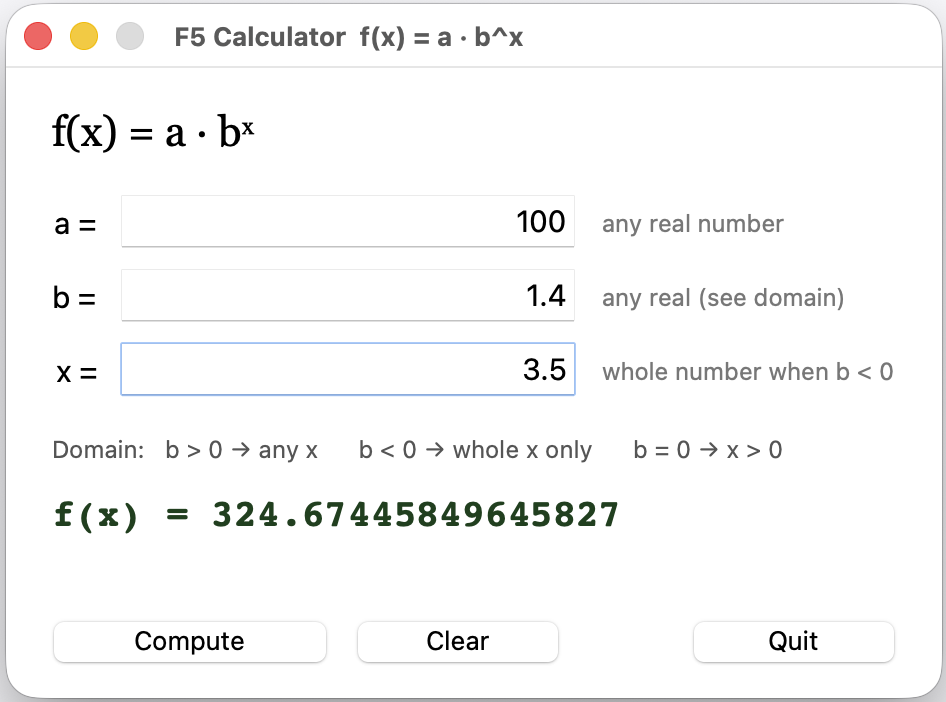
\includegraphics[width=\linewidth]{screenshot1.png}
      \end{center}
    \column{0.5\textwidth}
      \begin{center}
      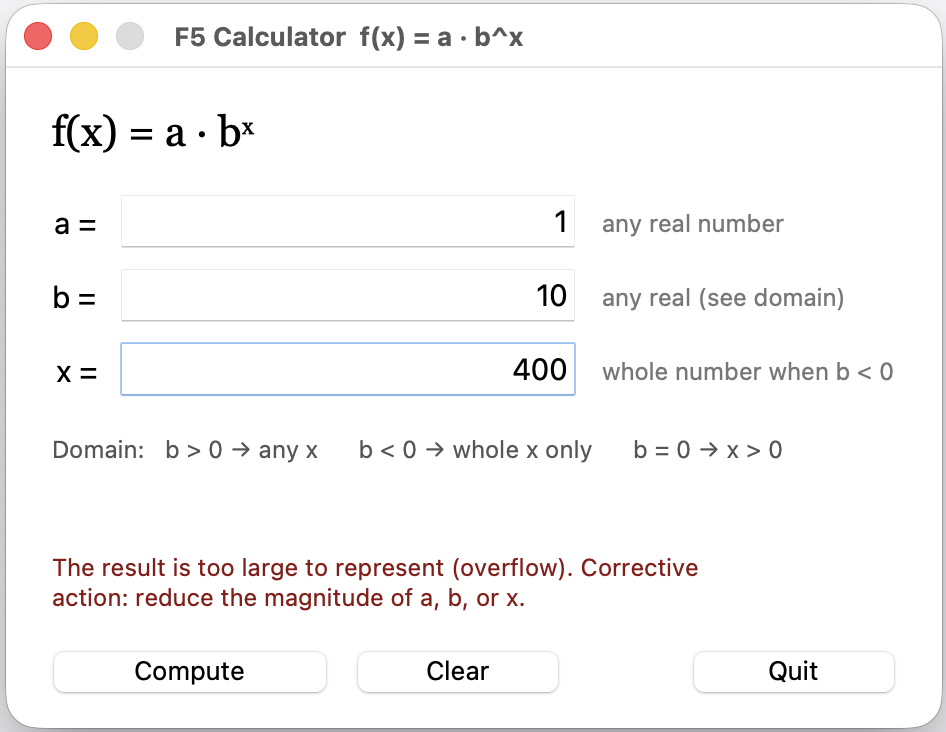
\includegraphics[width=\linewidth]{screenshot2.png}
      \end{center}
  \end{columns}
  \medskip
  \begin{itemize}
    \item Labelled fields for $a$, $b$ and $x$; Compute, Clear and Quit buttons;
          a result area.
    \item Input is checked before any computation runs, and an error is shown
          without closing the window. The persona's complaint was tools that
          simply die on overflow.
    \item New values can be entered straight away, with no restart (FR-06).
  \end{itemize}
\end{frame}

\begin{frame}{Problem 5: Demonstration Plan (ninety seconds)}
  \begin{enumerate}
    \item Normal growth case: $a = 100$, $b = 1.4$, $x = 3.5$ (the persona's scenario).
    \item Extreme base now accepted: $b = 10^{15}$ (this failed in D1).
    \item Negative base with a whole-number exponent: $a = 1$, $b = -2$, $x = 3$.
    \item Rejected input with a corrective message: $b = -2$, $x = 0.5$.
    \item Quit.
  \end{enumerate}
  \medskip
  Each case is there to show one requirement working: FR-02, the range
  reduction, FR-05, FR-04 with NFR-03, and FR-10.
\end{frame}

% ===============================================================
% PROBLEM 6 (20 marks): version control, commits, README
% ===============================================================
\begin{frame}{Problem 6: Version Control}
  \begin{columns}[T]
    \column{0.53\textwidth}
      \small
      \begin{itemize}
        \item Public repository:\\
              {\scriptsize\texttt{github.com/chandanpreet707/}\\
               \texttt{soen6011-f5-calculator}}
        \item One commit per function or concern. Each message has a short
              instruction-style subject line and a body saying \emph{why} the
              change was made, not just what changed.
        \item The repository also holds a flowchart for each function in
              \texttt{docs/flowcharts/}, the updated requirements in
              \texttt{docs/}, and a README with the module map and run
              instructions that need no installation.
      \end{itemize}
    \column{0.45\textwidth}
      \begin{center}
      % Crop to the two expanded commit bodies. Bounded on both axes so the
      % slide cannot overflow whatever crop ratio is used.
      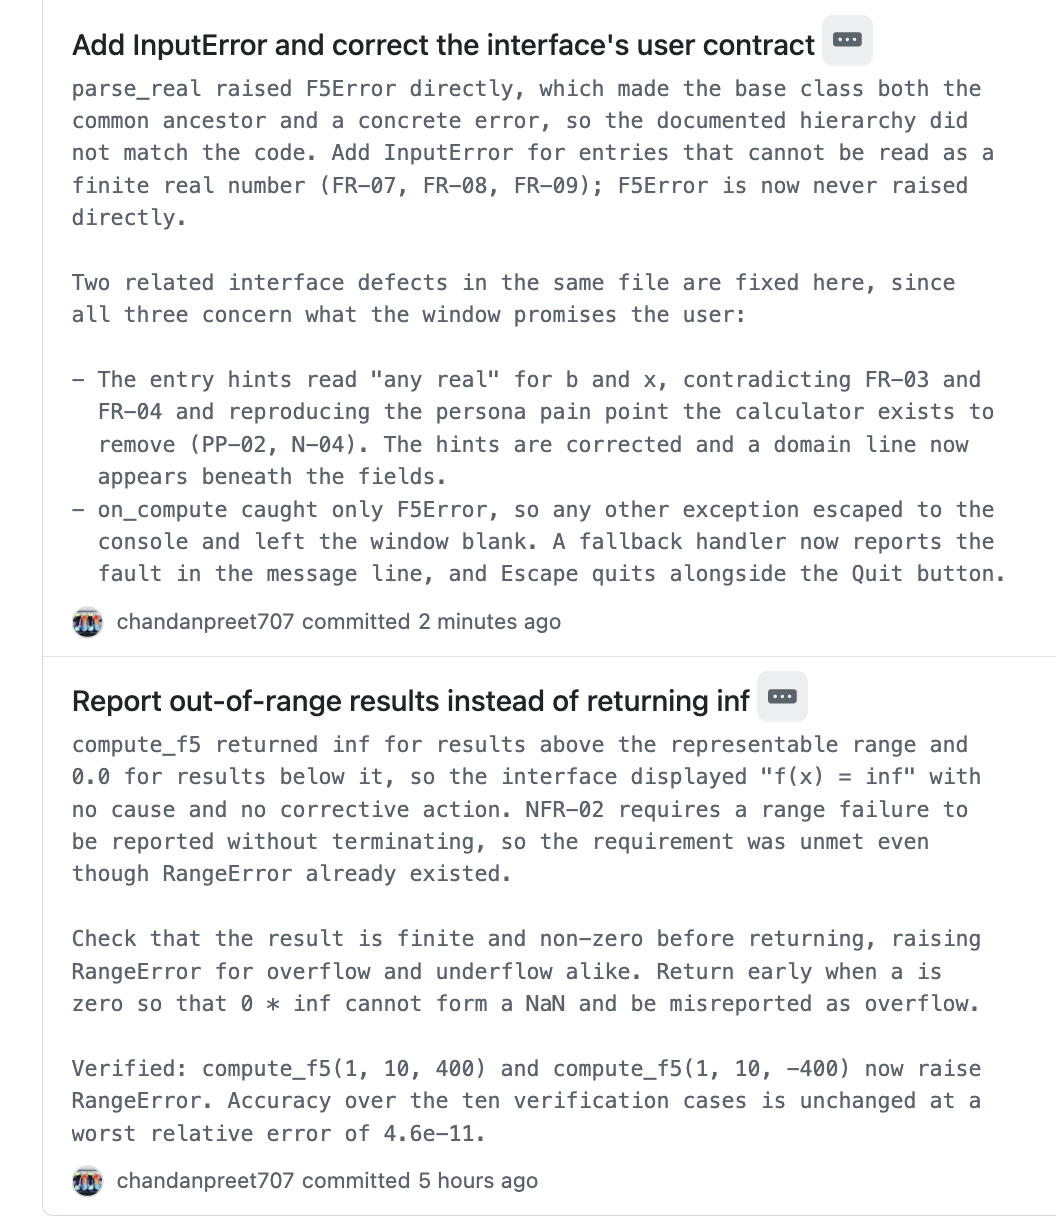
\includegraphics[width=\linewidth,height=0.70\textheight,keepaspectratio]{screenshot3.png}
      \end{center}
  \end{columns}
\end{frame}

% ===============================================================
% PROBLEM 7 (20 marks): updated requirements
% ===============================================================
\begin{frame}{Problem 7: How the Requirements Were Updated}
  \begin{itemize}
    \item The style is unchanged from D1: the ISO/IEC/IEEE 29148 construct
          [Condition] [Subject] shall [Action] [Object] [Constraint].
    \item Two things drove the update:
    \begin{itemize}
      \item \textbf{The D2 design.} The interface is now a GUI, and the
            from-scratch and exception rules are now stated as constraints.
      \item \textbf{A gap analysis of D1.} Behaviour that existed in the code
            but had no requirement covering it.
    \end{itemize}
    \item \textbf{Fixing the D1 trace problem.} In D1 the traces were phrases
          such as ``Goals'' and ``Pain Point 1''. Every persona element now
          has a unique identifier (\texttt{G-01}, \texttt{N-03}, \texttt{PP-01},
          and so on), and every requirement cites those identifiers.
          \texttt{FR-05} traced to ``Completeness'' in D1; it now traces to
          \texttt{PP-01} and \texttt{G-01}.
    \item The identifiers on these slides are the same ones written into the
          source-code docstrings, so the code and the requirements cannot drift
          apart.
    \item The complete updated list and the traceability matrix are appendix slides.
  \end{itemize}
\end{frame}

\begin{frame}{Problem 7: What Changed}
  \scriptsize
  \begin{itemize}
    \item \textbf{FR-07 (new).} When an entry is not a number in decimal
          notation, the F5 Calculator shall reject the input and display the
          cause and a corrective action.
          [\texttt{G-03}, \texttt{PP-02}, \texttt{N-04}]
    \item \textbf{FR-08 (new).} When an entry field is empty, the F5
          Calculator shall reject the input and display the cause and a
          corrective action. [\texttt{G-03}, \texttt{N-01}]
    \item \textbf{FR-09 (new).} When an entry is an infinite or
          not-a-number value, the F5 Calculator shall reject the input and
          display the cause and a corrective action.
          [\texttt{G-03}, \texttt{PP-03}]
    \item \textbf{FR-10 (new).} When the user activates the Quit control, the
          F5 Calculator shall close the application window and end the session.
          [\texttt{N-03}; demonstrated in D1, previously untraced]
    \item \textbf{NFR-04 (new).} When a series fails to converge within its
          iteration limit, the F5 Calculator shall report a convergence error
          without terminating. [\texttt{PP-03}, \texttt{PD-04}]
    \item \textbf{FR-05 (trace corrected).} Was ``Completeness''; now
          [\texttt{PP-01}, \texttt{G-01}].
    \item \textbf{NFR-02 (unchanged wording, now enforced).} A result outside
          the representable range is reported instead of returned as
          \texttt{inf} or zero. [\texttt{PP-03}]
    \item \textbf{DC-01 (revised).} Graphical user interface using Tkinter
          [was: textual interface]. [\texttt{PD-02}]
    \item \textbf{DC-02 (new).} Runs on a standard Python installation, with no
          administrator rights, IDE, or third-party package.
          [\texttt{PL-01}, \texttt{PD-03}]
    \item \textbf{DC-03 (new).} Uses no built-in or library function beyond
          input, output, arithmetic and interface design. [\texttt{PD-01}]
    \item FR-01--FR-06, NFR-01--NFR-03 and A1--A5 keep their D1 identifiers
          unchanged. New behaviour gets new identifiers; nothing is renumbered,
          so a D1 identifier still means the same thing in D2.
  \end{itemize}
\end{frame}

\begin{frame}{Summary}
  \begin{itemize}
    \item \textbf{Problem 5:} the function is computed entirely from scratch
          through five subordinate functions, with three measured improvements
          over D1, custom exception classes, and a Tkinter interface.
    \item \textbf{Problem 6:} a public repository with one commit per concern,
          a flowchart per function, and a README.
    \item \textbf{Problem 7:} the requirements were updated from the D2 design
          and from a gap analysis of D1, and every requirement now traces to a
          uniquely identified persona element.
  \end{itemize}
\end{frame}

% ===============================================================
\appendix
% APPENDIX SLIDES: required evidence, shown on request
% ===============================================================

\begin{frame}{Appendix: Persona Element Identifiers}
  \scriptsize
  These identifiers replace the D1 trace phrases. Each one is unique and is
  cited by at least one requirement.
  \begin{center}
  \begin{tabular}{ll}
    \toprule
    ID & Persona element (\'Elodie Tremblay, D1/Problem 1) \\
    \midrule
    \texttt{PL-01} & Managed Windows laptop; no admin rights; no IDE install \\
    \texttt{G-01} & Evaluate $ab^{x}$ repeatedly for many $(a,b,x)$ in one session \\
    \texttt{G-02} & Obtain at least six significant digits \\
    \texttt{G-03} & Understand why an input was rejected \\
    \texttt{N-01} & Clearly labelled inputs \\
    \texttt{N-02} & Precise results \\
    \texttt{N-03} & Fast repeated evaluation without restarting \\
    \texttt{N-04} & Guidance on the valid input ranges \\
    \texttt{PP-01} & Unhelpful errors when $b<0$ and $x$ is not an integer \\
    \texttt{PP-02} & No indication of the valid domain of $a$, $b$, $x$ \\
    \texttt{PP-03} & Overflow ends the tool with no explanation \\
    \midrule
    \texttt{PD-01} & Project description: implement from scratch \\
    \texttt{PD-02} & Project description: GUI using Tkinter \\
    \texttt{PD-03} & Project description: no dependence on an IDE \\
    \texttt{PD-04} & Project description: support for handling exceptions \\
    \texttt{PD-05} & Project description: error messages helpful to users \\
    \bottomrule
  \end{tabular}
  \end{center}
\end{frame}

\begin{frame}{Appendix: Full Updated Requirements (1 of 3)}
  \scriptsize
  \begin{itemize}
    \item \textbf{FR-01.} The F5 Calculator shall accept real values of $a$,
          $b$ and $x$ in decimal notation.
          [\texttt{N-01}, \texttt{G-01}]
    \item \textbf{FR-02.} When $b > 0$, the F5 Calculator shall compute
          $f(x) = ab^{x}$ for any real $x$. [\texttt{G-01}]
    \item \textbf{FR-03.} When $b = 0$ and $x \le 0$, the F5 Calculator shall
          reject the input and display the cause and a corrective action.
          [\texttt{PP-02}, \texttt{G-03}]
    \item \textbf{FR-04.} When $b < 0$ and $x$ is not an integer, the F5
          Calculator shall reject the input and display the valid domain of
          $x$ for a negative base.
          [\texttt{PP-01}, \texttt{N-04}, \texttt{G-03}]
    \item \textbf{FR-05.} When $b < 0$ and $x$ is an integer, the F5
          Calculator shall compute $f(x) = ab^{x}$.
          [\texttt{PP-01}, \texttt{G-01}]
    \item \textbf{FR-06.} Upon displaying a result, the F5 Calculator shall
          accept new values of $a$, $b$ and $x$ without requiring a restart.
          [\texttt{N-03}]  (D1 wording said ``prompt''; there are no prompts
          in a graphical interface.)
  \end{itemize}
\end{frame}

\begin{frame}{Appendix: Full Updated Requirements (2 of 3)}
  \scriptsize
  \begin{itemize}
    \item \textbf{FR-07.} When an entry is not a number in decimal notation,
          the F5 Calculator shall reject the input and display the cause and
          a corrective action.
          [\texttt{G-03}, \texttt{PP-02}, \texttt{N-04}]
    \item \textbf{FR-08.} When an entry field is empty, the F5 Calculator
          shall reject the input and display the cause and a corrective
          action. [\texttt{G-03}, \texttt{N-01}]
    \item \textbf{FR-09.} When an entry is an infinite or not-a-number
          value, the F5 Calculator shall reject the input and display the
          cause and a corrective action.
          [\texttt{G-03}, \texttt{PP-03}]
    \item \textbf{FR-10.} When the user activates the Quit control, the F5
          Calculator shall close the application window and end the session.
          [\texttt{N-03}]

  \end{itemize}
  \medskip
  \textbf{Assumptions (retained from D1).}
  \begin{itemize}
    \item \textbf{A1.} $a$, $b$ and $x$ are entered by the user for each
          evaluation, in decimal notation.
    \item \textbf{A2.} Exponents are treated as rational. To keep results
          real-valued, a non-integer exponent is rejected when $b < 0$.
          (Confirmed with the instructor.)
    \item \textbf{A3.} Only the principal real value of $ab^{x}$ is computed.
    \item \textbf{A4.} The language of interaction is English.
    \item \textbf{A5.} One user interacts with the calculator at a time.
  \end{itemize}
\end{frame}

\begin{frame}{Appendix: Full Updated Requirements (3 of 3)}
  \scriptsize
  \begin{itemize}
    \item \textbf{NFR-01.} The F5 Calculator shall compute results accurate to
          at least six significant digits.
          [\texttt{G-02}, \texttt{N-02}]
    \item \textbf{NFR-02.} When a computation exceeds the representable
          numeric range, the F5 Calculator shall display the cause and remain
          open for further input. [\texttt{PP-03}]
    \item \textbf{NFR-03.} Each error message shall state the cause of the
          error and a corrective action.
          [\texttt{PP-01}, \texttt{G-03}, \texttt{PD-05}]
    \item \textbf{NFR-02 (unchanged wording, now enforced).} A result outside
          the representable range is reported instead of returned as
          \texttt{inf} or zero. [\texttt{PP-03}]
    \item \textbf{NFR-04 (new).} When a series fails to converge within its
          iteration limit, the F5 Calculator shall report a convergence error
          without terminating. [\texttt{PP-03}, \texttt{PD-04}]
    \item \textbf{DC-01 (revised).} The F5 Calculator shall provide a
          graphical user interface implemented with Tkinter. [\texttt{PD-02}]
    \item \textbf{DC-02 (new).} The F5 Calculator shall run on a standard
          Python installation without administrator rights, an IDE, or
          third-party packages. [\texttt{PL-01}, \texttt{PD-03}]
    \item \textbf{DC-03 (new).} The implementation shall use no built-in or
          library functions beyond those for input, output, arithmetic, and
          user interface design. [\texttt{PD-01}]
  \end{itemize}
\end{frame}

\begin{frame}{Appendix: Traceability, Both Directions}
  \scriptsize
  Every requirement cites a source, and every persona element is covered by at
  least one requirement. This is the check the D1 marker asked for.
  \begin{center}
  \begin{tabular}{ll}
    \toprule
    Source element & Requirements that cover it \\
    \midrule
    \texttt{PL-01} & DC-02 \\
    \texttt{G-01} & FR-01, FR-02, FR-05 \\
    \texttt{G-02} & NFR-01 \\
    \texttt{G-03} & FR-03, FR-04, FR-07, FR-08, FR-09, NFR-03 \\
    \texttt{N-01} & FR-01, FR-08 \\
    \texttt{N-02} & NFR-01 \\
    \texttt{N-03} & FR-06, FR-10 \\
    \texttt{N-04} & FR-04, FR-07 \\
    \texttt{PP-01} & FR-04, FR-05, NFR-03 \\
    \texttt{PP-02} & FR-03, FR-07 \\
    \texttt{PP-03} & FR-09, NFR-02, NFR-04 \\
    \texttt{PD-01}     & DC-03 \\
    \texttt{PD-02}     & DC-01 \\
    \texttt{PD-03}     & DC-02 \\
    \texttt{PD-04}     & NFR-04 \\
    \texttt{PD-05}     & NFR-03 \\
    \bottomrule
  \end{tabular}
  \end{center}
  No requirement is left without a source, and no persona element is left
  without a requirement.
\end{frame}

\begin{frame}{Appendix: Subordinate Function Details, \texttt{ln}}
  For $m \in [1,2)$ and $t = (m-1)/(m+1)$:
  \[ \ln b = 2 \sum_{k=0}^{\infty} \frac{t^{2k+1}}{2k+1} + p \ln 2,
     \qquad b = m \cdot 2^{p} \]
  \begin{itemize}
    \item Because $m$ is between 1 and 2, $|t| \le 1/3$, which is what makes
          the series converge quickly for every base.
    \item $\ln 2$ is computed once by the same series. Nothing is taken from a
          table of constants.
    \item The iteration cap raises \texttt{ConvergenceError}, so the loop can
          never run forever.
    \item Measured relative error is at most about $2 \times 10^{-12}$ against
          the reference implementation, across $b \in [10^{-15}, 10^{15}]$.
  \end{itemize}
\end{frame}

\begin{frame}{Appendix: Subordinate Function Details, \texttt{exp} and \texttt{pow\_int}}
  \begin{itemize}
    \item \texttt{exp}: Maclaurin series, each term built from the previous
          one. Negative arguments go through $e^{y} = 1/e^{-y}$ to avoid
          catastrophic cancellation. At $y = -30$ the D1 error was a factor of
          $6\times10^{7}$; D2 is about $3\times10^{-16}$.
    \item \texttt{pow\_int}: exponentiation by squaring, meaning the exponent
          is halved at each step, so $O(\log n)$ multiplications instead of
          $n$. Whole-number results come out exact.
    \item Worked examples and a flowchart for each of the five functions are in
          \texttt{docs/flowcharts/} in the repository.
  \end{itemize}
\end{frame}

\begin{frame}{Appendix: Verification Evidence}
  \scriptsize
  \begin{center}
  \begin{tabular}{rrrr}
    \toprule
    $a$ & $b$ & $x$ & relative error \\
    \midrule
    2   & 3         & 2.5  & $6.0\times10^{-13}$ \\
    100 & 1.4       & 3.5  & $1.5\times10^{-13}$ \\
    1   & 2         & 10   & exact ($1024.0$) \\
    5   & 10        & 0.5  & $1.6\times10^{-12}$ \\
    1   & 0.5       & 3.5  & $5.2\times10^{-13}$ \\
    2   & 7         & 3.25 & $5.6\times10^{-13}$ \\
    1   & $10^{15}$ & 0.9  & $4.6\times10^{-11}$ \\
    1   & $-2$      & 3    & exact ($-8.0$) \\
    3   & $-2$      & 4    & exact ($48.0$) \\
    1   & $-2$      & 0    & exact ($1.0$) \\
    \bottomrule
  \end{tabular}
  \end{center}
  \normalsize
  \footnotesize
  Ten accuracy cases, extended from the nine used in D1. Worst relative error
  $4.6\times10^{-11}$, satisfying NFR-01 (six significant digits).
  \texttt{verify\_f5.py} also exercises five rejection cases (FR-03, FR-04,
  and NFR-02 overflow and underflow) and reports whether each was refused.
  The built-in \texttt{**} appears only in that script, as the oracle; the
  calculator itself uses none of it, so DC-03 holds.
\end{frame}

% ===============================================================
% GAI / CASTROFF documentation (required for every problem)
% ===============================================================
\begin{frame}{Appendix: GAI Usage, Approach}
  \begin{itemize}
    \item Tool used for all three problems: Claude (Anthropic), a publicly
          available assistant based on a large language model.
    \item Prompts follow the CASTROFF framework: Constraints, Audience,
          Structure, Tone, Role, Output format, Focus, Function.
    \item Workflow: prompt, output, human review, refinement, verification.
          Nothing was accepted until it had been tested against a reference.
  \end{itemize}
\end{frame}

\begin{frame}{Appendix: GAI Usage, Problem 5}
  \textbf{Prompt types:} implementation from a specification; defect analysis.
  \medskip

  \textbf{Example prompt:} ``Acting as a numerical software engineer [Role],
  implement a natural logarithm from scratch in Python [Focus] without any
  library functions [Constraints], using the atanh series with range
  reduction so that extreme bases converge quickly [Function], with
  docstrings explaining the mathematics for a graduate evaluator
  [Audience, Tone], as a single module [Structure, Output format].''
  \medskip

  \textbf{Output evaluation:} \emph{Accepted} the range-reduction structure.
  \emph{Corrected} the constant handling so that $\ln 2$ is computed by the
  series rather than tabulated. \emph{Rejected} the first \texttt{exp}
  version once testing exposed catastrophic cancellation for negative
  arguments, and required the reciprocal form instead. All accepted code was
  verified against a reference implementation before use.
\end{frame}

\begin{frame}{Appendix: GAI Usage, Problems 6 and 7}
  \small
  \textbf{Problem 6 (repository).} Prompt type: review and generation.
  Example: ``As a maintainer [Role], write high-quality commit messages
  [Focus] with an instruction-style subject and a body explaining the reason
  for the change [Structure], and a README for a from-scratch calculator
  [Function], for a graduate evaluator [Audience], in plain technical English
  [Tone], without marketing language [Constraints].''
  \emph{Accepted} the commit-message structure. \emph{Corrected} the claims so
  that every stated number matches a measured value. \emph{Rejected} filler
  wording.
  \medskip

  \textbf{Problem 7 (requirements).} Prompt type: transformation with gap
  analysis. Example: ``As a requirements engineer [Role], update the D1
  requirements from the D2 code and the marker feedback [Focus], giving each
  persona element a unique trace identifier [Structure, Constraints], in
  ISO/IEC/IEEE 29148 style [Output format], for the instructor [Audience],
  objectively [Tone], covering malformed input, quitting, and the difference
  between non-convergence and overflow [Function].''
  \emph{Accepted} the identifier scheme and the new traces. \emph{Corrected}
  the FR-05 trace by hand. \emph{Verified} that every requirement traces in
  both directions before accepting the result.
\end{frame}

\begin{frame}{Appendix: References}
  \footnotesize
  \begin{thebibliography}{9}
    \bibitem{cormen} T. H. Cormen, C. E. Leiserson, R. L. Rivest, and
      C. Stein, \emph{Introduction to Algorithms}, 4th ed. Cambridge, MA,
      USA: MIT Press, 2022. (Exponentiation by squaring; pseudocode format.)
    \bibitem{stewart} J. Stewart, \emph{Calculus: Early Transcendentals},
      8th ed. Boston, MA, USA: Cengage Learning, 2015. (Maclaurin series;
      atanh series for the logarithm.)
    \bibitem{goldberg} D. Goldberg, ``What every computer scientist should
      know about floating-point arithmetic,'' \emph{ACM Computing Surveys},
      vol. 23, no. 1, pp. 5--48, 1991. (Catastrophic cancellation; range
      reduction.)
    \bibitem{iso29148} \emph{Systems and Software Engineering: Life Cycle
      Processes: Requirements Engineering}, ISO/IEC/IEEE Std. 29148, 2018.
    \bibitem{castroff} H. Tavakoli, ``The CASTROFF framework: A professional
      standard for prompt engineering,'' in \emph{Prompt Engineering for
      Everyone}. Berkeley, CA, USA: Apress, 2026, ch. 6, pp. 95--116.
    \bibitem{python} Python Software Foundation, \emph{Python 3
      Documentation}. [Online]. Available: https://docs.python.org/3/
      (Reference implementation for verification test cases;
      Tkinter documentation.)
  \end{thebibliography}
\end{frame}

\end{document}